% After studying the \numissues data constraint issues reported in the applications' bug-tracking systems, 
 We categorize \numissues real-world issues 
 into 4 types as shown in Table \ref{tab:issuecat}.
 
 \iffalse 
 :
 (1) data constraints located at different software components conflict with
 each other (WHERE issue); (2) the exact requirement imposed by a data constraint
 conflicts with what the users or the application logic actually expects 
 (WHAT issue); (3) data constraints specified in different code versions conflict
 with each other (WHEN issue); and (4) a constraint's violation-checking result
 is not properly delivered to web users (HOW issue).
 \fi 



\subsection{WHERE is the constraint specified?}
\label{subsec:where}
As discussed, application and DB constraints for the same data field can be inconsistent with each other. Such inconsistencies contributed to 24 out of the 114 issues.

\paragraph{\bf Application constraints looser than DB constraints} 13 out of 24 issues fall into this category. In 12 of them, the constraint is completely missing in application layer while the rest one issue happens because the length constraint has a smaller value in database layer than in application layer.
In these cases, a record saving operation would pass the application server's
checking but fail in the DB, causing a web page crash
with an unhandled raw DB error thrown to end users, which is
often difficult to understand and causes poor user experience. The example discussed in 
Figure \ref{fig:crossstack} is an illustration. 

\paragraph{\bf Application constraints stricter than DB constraints} 11 out of 24 issues fall into this category. In 9 of them, application constraints are not defined in database layer at all while the rest two are caused by that length constraint has smaller value in application layer than in database layer.  
In these cases, the application misbehaves as the administrator/user
directly 
%\shan{who exactly can issue SQL request to DB server directly?}
changes database records through SQL queries in a way that violates application constraints. This happens quite often.   For example, Spree \cite{spree}, an on-line shopping system, has 4 issues caused by administrators modifying database content through direct SQL requests. Discourse \cite{discourse} even has scripts that bypass model constraints to import other forum applications' data. 

Figure~\ref{fig:spree-3829-different} shows such an issue~\cite{spree-3829} in Spree. As shown in (b), each {\tt LineItem} is associated with a {\tt variant} object and a {\tt presence} constraint is used to ensure the existence of every associated {\tt variant}. This ensures that an expression like
{\tt item.variant.image} in (a) is never null.
%Specifically, this presence constraint is checked whenever an {\tt LineItem} object is saved by the application, and it would cause the saving to fail if the associated {\tt variant} object does not exist. 
However, this constraint does not exist in the database. In this bug report,
an adminstrator accidentally deleted a {\tt variant} record in the DB
that is associated with a {\tt LineItem} record, and that
led to a null pointer error when he tried to display 
an order through the code in Figure~\ref{fig:spree-3829-different}a. 
%In the spree issue, only admin users will be affected by the corrupted data. However, there are other issues such as Discourse-30278 in which normal users suffer from null-pointer errors with page crashes because one post's topic has been deleted. 

\begin{table}[]
\centering
\caption{Data-constraint issues in real-world apps}
\label{tab:issuecat}
\setlength{\tabcolsep}{4pt}  
\resizebox{0.6\columnwidth}{!}{
% \begin{tabular}{lrrrrrr}
% \toprule 
% & WHERE
% &  \multicolumn{2}{c}{WHAT}   & WHEN  & HOW & SUM  \\ 
% \cmidrule{3-4}
% & 
% &  vs. code  & vs. user  &   &  &   \\ 
% \midrule
% Ds  & 3  & 0  & 6  & 2  & 2  & 13  \\ \midrule
% Lo  & 0  & 1  & 0  & 0  & 0  & 1   \\ \midrule
% Gi  & 3  & 8  & 0  & 4  & 1  & 16  \\ \midrule
% Re  & 7  & 11 & 4  & 1  & 7  & 30  \\ \midrule
% Sp  & 8  & 14 & 3  & 3  & 3  & 31  \\ \midrule
% Ro  & 0  & 1  & 1  & 0  & 0  & 2   \\ \midrule
% Fu  & 1  & 0  & 0  & 0  & 0  & 1   \\ \midrule
% Tr  & 0  & 0  & 1  & 1  & 0  & 2   \\ \midrule
% Da  & 0  & 4  & 1  & 1  & 5  & 11  \\ \midrule
% On  & 2  & 2  & 1  & 0  & 0  & 5   \\ \midrule
% FF  & 0  & 0  & 0  & 0  & 0  & 0   \\ \midrule
% OSM & 0  & 0  & 0  & 0  & 2  & 2   \\ \midrule
% SUM & 24 & 41 & 17 & 12 & 20 & 114 \\ \bottomrule
% \end{tabular}

\begin{tabular}{@{}rrrrrrrrrrrrrrr@{}}
\toprule
                      &          & Ds & Lo & Gi & Re & Sp & Ro & Fu & Tr & Da & On & FF & OSM & SUM \\ \midrule
WHERE                 &          & 3  & 0  & 3  & 7  & 8  & 0  & 1  & 0  & 0  & 2  & 0  & 0   & 24  \\ \midrule
\multirow{2}{*}{WHAT} & vs. code & 0  & 1  & 8  & 11 & 14 & 1  & 0  & 0  & 4  & 2  & 0  & 0   & 41  \\ \cmidrule(l){2-15} 
                      & vs. user & 6  & 0  & 0  & 4  & 3  & 1  & 0  & 1  & 1  & 1  & 0  & 0   & 17  \\ \midrule
WHEN                  &          & 3  & 0  & 4  & 1  & 3  & 0  & 0  & 0  & 1  & 0  & 0  & 0   & 12  \\ \midrule
HOW                   &          & 2  & 0  & 1  & 7  & 3  & 0  & 0  & 0  & 5  & 0  & 0  & 2   & 20  \\ \midrule
SUM                   &          & 14 & 1  & 16 & 30 & 31 & 2  & 1  & 1  & 11 & 5  & 0  & 2   & 114 \\ 


\bottomrule
\end{tabular}
}
\footnotesize{}
\end{table}


\begin{figure}
    \centering
    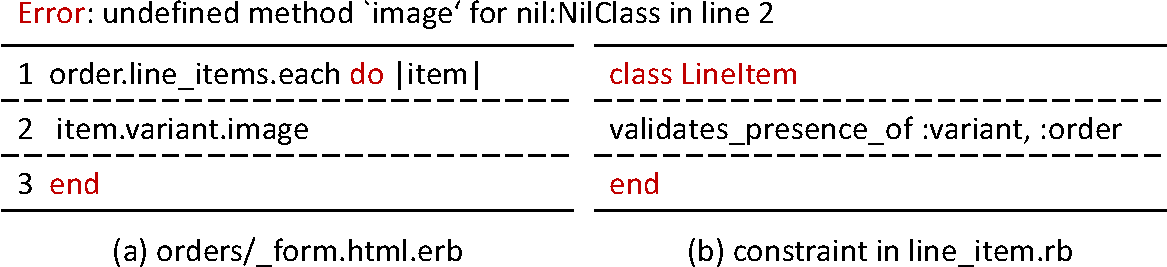
\includegraphics[width=0.6\columnwidth]{constraints/figs/spree-3829-different2.pdf}
    
    \caption{Constraint mismatch in Spree}
    
    \label{fig:spree-3829-different}
\end{figure}

% The could also be incompatibility between html layer and model 

% \junwen{We don't have issues caused by inconsistency of html constraint and model constraint. If there is, the symptom would be  misleading error message. }
% \shan{I remember you started looking into html-end constraint because you saw some
% inconsistency. right?}

\paragraph{\bf Summary}
As shown by real-world issues, inconsistencies between application 
 and database constraints cause problems, including
web page crashes and poor user experience.
Considering the hundreds and thousands of constraints that exist in the DB
but not in application and vice versa 
(see Section~\ref{sec:one_where}), 
this problem could be much more severe and widespread than
what reflected by the issue reports.
Automatically detecting such constraint inconsistencies will be very helpful, which we further explore in Section \ref{sec:solution}.

\subsection{WHAT is the constraint about?}
\label{subsec:what}
The most common problem is a mismatch between how data is supposed to be used in the application and the constraints imposed on it. This accounts for 
58 out of \numissues issues. 
%\alvin{i don't quite get what you mean. you mean conflict between constraints specified in app vs constraints specified in the db?}\shan{no, it is like the constraint said this should be an integer, but the application tries to get the square root of this data, which indicates the constraint should positive-integer, not just integer.}


\subsubsection{{Conflict with user needs}}

Users sometimes would relax an existing constraint,
such as increasing the input length of name field in tracker from 30 to 100 (Redmine-23235 \cite{redmine-25235}).
These contribute to about 10\% of the issues in our study.
%Another user in Tracks asks ``The passwords are limited to 40 characters.
%I don't like the limit, so is it possible to increase it?''. 
%The solution is simple as shown in Figure~\ref{fig:tracks-1921-passwordlength}, 
%in Discourse-79684: ``On our site users sometimes want really long `About Me' descriptions in their profiles but it is by default limited to 3000 characters. Is there any easy way to bump this up?''.
%Similarly, a user posted an issue in Discourse \cite{discourse.75453}, saying ``Does anyone know if there is a way to modify the maximum character limit for category names? I need to ...".
%put an English title, followed by the French equivalent, but I am running out of room to do both.''. 
Developers usually satisfy the users' desires and change constraints
accordingly. 

\iffalse
In Redmine, the corresponding length-constraint was only
specified in application, not in DB, and the patch simply changed
the application validation function parameter to allow longer
inputs; in Discourse, since Category-name has its length constraint
specified in both application and in DB, the patch changed
both places.
\fi 

% Sometimes, the constraints validation needs to be skipped. For example, in Spree-7389, user says ``There is validation for Address model for zipcode. It's always check it even though this may be problem because for example Hong Kong doesn't have zipcodes.''

\iffalse 
\begin{figure}
    \centering
    \includegraphics[width=0.8\columnwidth]{figs/tracks-1921-passwordlength.pdf}
    \caption{Too tight constraint in Tracks}
    \label{fig:tracks-1921-passwordlength}
    %link: https://github.com/TracksApp/tracks/issues/1921
\end{figure}
\fi 

\paragraph{\bf Summary}  For certain type of constraints, like the
length constraint, it is difficult to have one setting that satisfies all users' needs. It would be helpful if refactoring routines can be designed to turn a fixed-setting constraint into configurable. %\shan{1.none of your example above is about configurable; 2.it is better to suggest some automation, like suggesting refactoring that makes some constraints that involve numerical bounds to be user configurable.}. 


\subsubsection{{Conflict with application needs}}
\label{sec:what_app}
Many constraints are created to guarantee program invariants
that are crucial to applications' functional correctness. 
Constraints that are insufficient or even conflicting with how the corresponding
data is used by the application contribute to more than one third of all the issues
in our study.

\paragraph{\textbf{Type conflicts}}
These constraints treat a data field as having a general type, but
the application uses the data field in a more specialized way
that demands tighter constraints. In one Redmine issue~\cite{redmine-9394}, a user noticed that she can input  invalid dates like
``2011-10-33'' without triggering any errors. 
This problem happened because Redmine only used a regular expression ``\textbackslash d\{4\}-\textbackslash d\{2\}-\textbackslash d\{2\}\textdollar'' to make sure the input follows the ``yyyy-mm-dd'' format without more detailed checking.
To solve this problem, Redmine later added ``value.to\_date'' to check whether the input   can really be converted to a date or not in the custom validate function shown in Figure~\ref{fig:redmine-9394-tooloose}.  

\begin{figure}
    \centering
    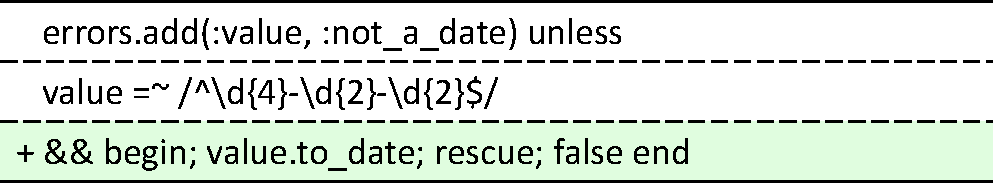
\includegraphics[width=0.6\columnwidth]{constraints/figs/redmine-9394-tooloose.pdf}
    \vspace{-0.2in}
    \caption{Type conflict example in Redmine}
    %\vspace{-0.1in}
    \label{fig:redmine-9394-tooloose}
\end{figure}

\textbf{Case sensitivity conflicts.} 
{\it Uniqueness} is a common constraint associated with a data field to
avoid duplication, like preventing two users from having the same ID. 
A common problem is that a field is written to the DB in
a case-sensitive way of uniqueness, while used or searched in a
case-insensitive way, or vice versa. Such inconsistency can lead to severe software misbehavior. 

In a Gitlab issue~\cite{gitlab-24493}, a user's profile email is all in lower case, but she committed code with an upper-case letter in her email, which then cannot
be matched to her profile. What is annoying was that she was 
unable to add the different casing as an alias, as Gitlab said
the email was ``already in use.''  This happens because when a user-email is stored into DB, the uniqueness checking
is case insensitive---``abc@example.com'' is treated the same as ``ABC@example.com.'' However, when the application searches for code commit using email
as the index, the search is case sensitive --- code committed by
``ABC@example.com'' cannot be retrieved by a search using
``abc@example.com.'' The patch made the search also
case insensitive, thus always converting the input email to pure-lowercase before the
search, as shown in Figure~\ref{fig:gitlabcasesensitive}. 

\begin{figure}
    \centering
    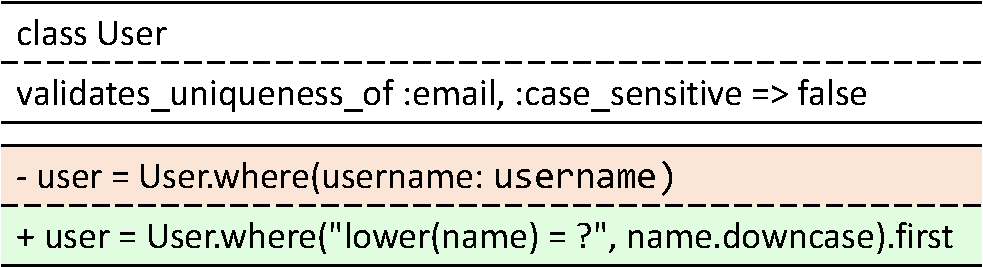
\includegraphics[width=0.6\columnwidth]{constraints/figs/gitlab-issue.pdf}
    \caption{Case sensitivity conflict example in Gitlab}
    %\vspace{-0.1in}
    \label{fig:gitlabcasesensitive}
\end{figure}

\textbf{Boundary value conflicts.} There are cases where certain
values of a data field are allowed by the application logic, 
but disallowed by the constraints. For example, in the typical checkout flow of Spree, users would enter their delivery details, then proceed to a payments page to enter discounts and payment details, and then finally arrive at a confirmation page. However, in one Spree issue\cite{spree-6673}, a user complained that when she entered a discount coupon that reduced the price to zero---which was actually a valid use case---the application did not allow him to proceed, and instead redirected back to the delivery page. The source of the bug was a constraint in the model layer ({\tt models/spree/order.rb}) which
%, in order to proceed to the next stage of the checkout flow, 
incorrectly required the value of the {\tt total} field to be strictly greater than zero.

\iffalse 
\begin{figure}
    \centering
    \includegraphics[width=\columnwidth]{figs/spree-issue.pdf}
    %\vspace{-0.1in}
    \caption{Boundary value inconsistency in Spree}
    \label{fig:spreerwinconsistency}
\end{figure}
\fi 

\paragraph{\bf Summary}
Failure symptoms of these bugs are quite different from all the other types 
of bugs (WHERE, WHEN, HOW). They can lead to severe software misbehavior or even
disable an entire feature of a web application.  
It would be ideal if a program analysis tool can compare how a data field
is used in software and identify inconsistency between how it is used and 
how it is constrained. This is challenging for generic data
types and data usage, but is feasible for specific types of 
problems, which we explore
in Sec. \ref{sec:solution}.


\subsection{WHEN is the constraint created?}
\label{subsec:when}

When upgrading an application, sometimes newly added or changed constraints might be incompatible with old data. 
12 issues are caused by such inconsistency across versions. 
The failure symptoms vary based on the different program context where the 
tighter constraint is checked.

\paragraph{\textbf{Read path}}
When a constraint is newly created or tightened along a DB-record loading code
path (e.g., front-end
constraint or application sanity-check changes), an  
incompatible new constraint can cause failures in
loading old data and hence severe functionality problems.
The Diaspora example in Section~\ref{sec:intro} belongs to this
category: the password's length requirement tightened and hence invalidated many old passwords.

\iffalse 
In the old version of Diaspora, it is allowed to set the password with length smaller than three. In one commit, developers have added an constraint in HTML level with format ``......+'' which limits the password  to be equal or longer than 6 characters. This causes many users, whose
passwords are shorter than 6 character, to fail to login to Diaspora with the 
unhelpful error-information saying ``Please use the required format''. 
Their solution is to remove the newly added constraints on the password length.


\begin{figure}
    \centering
    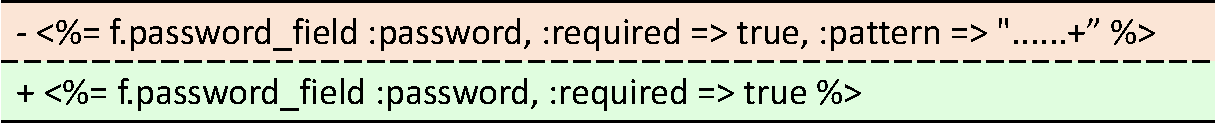
\includegraphics[width=\columnwidth]{figs/diaspora-4221-password.pdf}
    \vspace{-0.2in}
    \caption{Old data conflicts with new constraints (Diaspora)}
    \label{fig:diaspora-4221-password}
\end{figure}
\fi 

\paragraph{\textbf{Write path}}
When a constraint is newly created or tightened along a path that intends to
save a record to the database (e.g., all the application-validation constraints
and database constraints), the incompatibility between the new constraint
and old data can be triggered under the following two circumstances.
 

First, all the old data in the database will be checked against the new set 
of DB constraints during a migration process during
application upgrade. 
Inconsistency between old data and new DB constraints can cause an upgrade failure.
For example,
one Gitlab issue~\cite{gitlab-36919} complains that they failed to upgrade from version 9.4.5 to 9.5.0 due to {\tt NotNullViolation} during data migration. As shown in Figure~\ref{fig:gitlab-36919-when}, the {\tt decription\_html} column was added 
to Gitlab before version 9.4.5 (in the ``20160829...'' migration file) and was filled with {\tt null}s by 
default.\footnote{When no default value is specified in {\tt add\_column}, {\tt null} is used as the default value.}
% in migration add\_markdown\_cache\_columns.rb before 9.4.5, but the column still has null value
Later on, in the ``20170809...'' migration (shown in the Figure~\ref{fig:gitlab-36919-when}), a non-null constraint 
was added to the column through the API {\tt change\_column\_null} with parameter {\tt false}. This caused 
many users' upgrade to fail because there were many old records with
a default {\tt null} in that column. 
%There are two solutions to solve this issue, one is to change the constraint, 
The patch removed the ``non null'' constraint to the {\tt description\_html} column, as shown in 
Figure~\ref{fig:gitlab-36919-when}. 
%Of course, an alternative solution is to set a not-null default value for the column as shown in Figure~\ref{fig:gitlab-36919-when}.
%--edit to here
%We have also seen cases where the migration file added a new column with a {\tt not-null} constraint without setting default value for it. As a result, the system by default fills the new column with {\tt null} and immediately leads to migration/software-upgrade errors such as that in Gitlab-46862. 


Second, even if all the old data is validated against DB constraints and the application has successfully upgraded, the old data might still conflict
with new constraints specified through the application validation APIs that did not exist in the prior version.
This can lead to problems when the application allows users to edit an existing
 record---users may have trouble in saving an edited record back.
In one Discourse issue~\cite{discourse-89148}, a user complained that she made a small edit to an old post's  title, but was unable to save with an error message stating that the title was invalid.
It turned out that, the 
title's length constraint has been changed from 30
 to 20 characters in the application's validation function. That old post's title contained
28 characters; the small edit did not change the title length. So, the old post can still be loaded by the application, but cannot be saved back after such small edits.
 

 

\begin{figure}
    \centering
    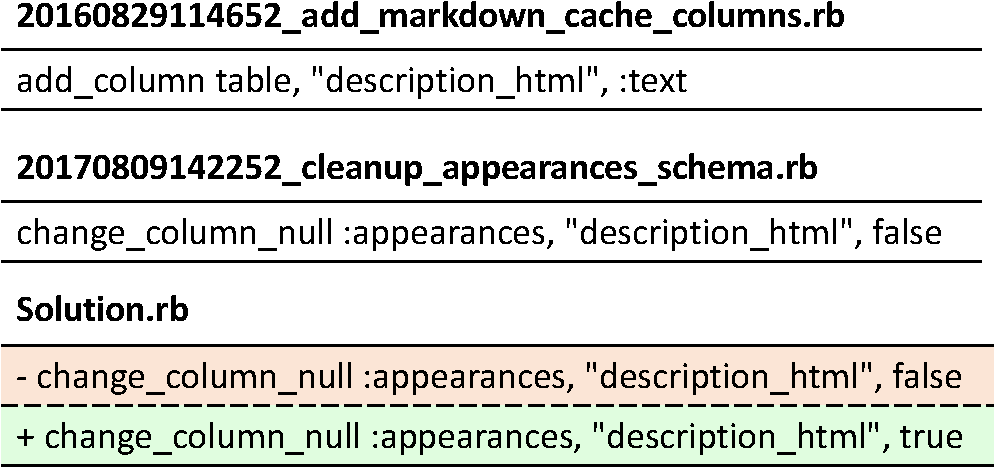
\includegraphics[width=0.6\columnwidth]{constraints/figs/gitlab-36919-when.pdf}
    \caption{Old data conflicts with new constraints in Gitlab}
    %\vspace{-0.1in}
    \label{fig:gitlab-36919-when}
\end{figure}

\paragraph{\bf Summary}  Given the frequent constraint addition and changing
in web applications, it is inevitable that old data may
become incompatible with new constraints. It would be helpful if automated 
tools can provide warnings for developers when constraints become
tighter in a new version, particularly (1) if the migration file has high probability to
fail (e.g., specifying a constraint that conflicts with a column's default value), then developers should fix the migration
file; (2) if the application allows editing old data, then developers should probably 
add explicit warning to users about the risk of editing old data; and finally
(3) the case of having tighter constraints that limit the reading of old data should be avoided. We explore this in Section~\ref{sec:solution}.

\subsection{HOW are the checking results delivered?}
%\utsav{Possibly include results on what portion of custom validations might be missing errors}
\label{subsec:how}

Constraint violation is common in web applications, as web users cannot anticipate all the constraints
in advance and will inevitably input constraint-violating data. Consequently,
delivering informative and friendly error messages is crucial to web applications'
user experience. 20 issues in our study are about this problem. 
 
These 20 issues are mostly related to application-validation constraints.
Rails validation APIs provide default error messages that are mostly 
clear.\footnote{Section~\ref{sec:solution} discusses cases when the default message is unclear
and how we enhance it.} However, developers 
sometimes forgot to display the error message associated with the validation
APIs (8 cases) and sometimes override the default message with
uninformative generic messages (12 cases), which led to user complaints.
For example,
in a Diaspora issue~\cite{diaspora-5090}, a user complained that when he tried to post a long article, the posting failed with an unhelpful error message ``Failed to post!'' 
%The user demanded ``a more descriptive error message''. 
Developers found out that their code in {\tt posts\_controller} forgot to render the error message
defined in {\tt post}'s validation function. The patch fixed this problem
and would display the required length limit,
as shown in Figure~\ref{fig:diaspora-5151-errormsg}.
%\shan{Junwen, please make the patch figure simpler, only
%reflecting the change to show the length limit.}
%by ``please make your post less than 65536 characters''. Although this is not the default error message provided by Rails, the information revealed is the same. 
%In this particularly case, users later further requested to know not only the post limit but also the length of their failed submission, which was satisfied by later patches. 
%So eventually the error message was changed to ``Please make your post fewer than 65536 characters. Right now it is \%\{length\} characters'', in which  \%\{length\} is the current length of users' input post.
\begin{figure}
    \centering
    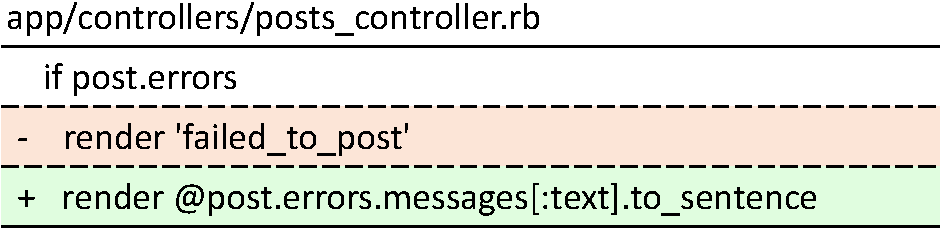
\includegraphics[width=0.6\columnwidth]{constraints/figs/diaspora-5990-errormsg-cp.pdf}
    \caption{Unclear error message in Diaspora}
    \label{fig:diaspora-5151-errormsg}
    %link: https://github.com/diaspora/diaspora/issues/2481
\end{figure}

\paragraph{\bf Summary} Developers should be reminded to display error messages associated with validation APIs. Future IDEs should automatically 
synthesize default error checking and error-message display code. 
Improving the quality of default and custom error message is crucial to
user experience. We will explore this in Section~\ref{sec:solution}.
%Some issues however requires a better understanding of the application behavior facing errors.
 

% \iffalse
% In Diaspora-2481, many users complain that they tried many times to reset password but failed with a bunch of error messages as shown in Figure~\ref{fig:diaspora-2481-unclear}~(b), which is very confusing since in the password reset page, there are only two fields for the new password and confirmation of it. There is no email and username on that page at all, not to mention the error message. The developer figured out this happens because the email address has been invited to Diaspora, but hasn't accepted the invitation yet, which is not reflected through the error message at all. And do not underestimate the importance of the error message. They are crucial to the popularity of the applications. A user says ``I had no idea what those messages meant, and a normal user would simply abandon their account.''. \shan{yeah, this
% bug is interesting. However, are we doing anything to help resolve this problem?
% the problem here seems to be that the error message is complaining about a field
% that the user entered in a previous page, right? That seems to be different
% from the problem you guys worked on?}

% \begin{figure}
%     \centering
%     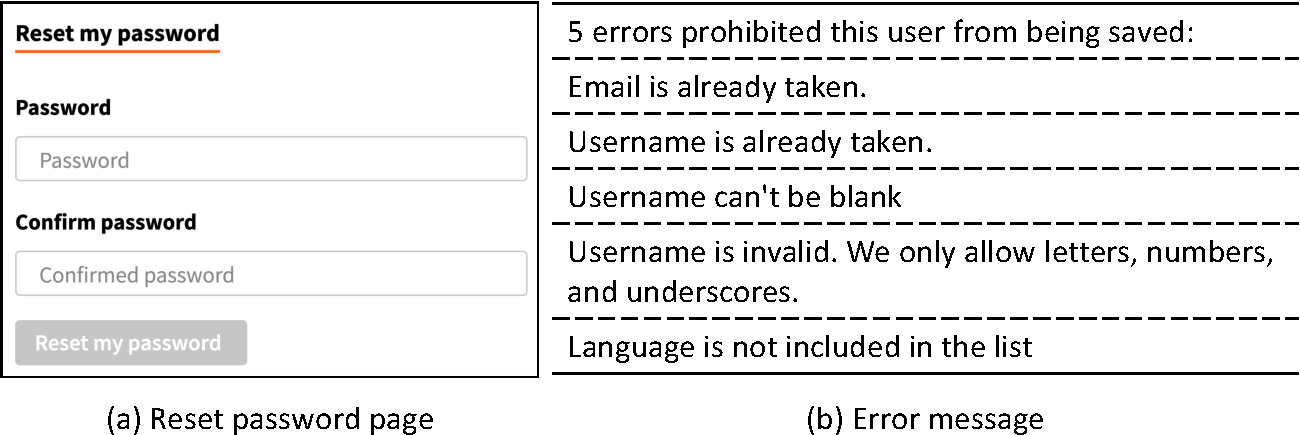
\includegraphics[width=\columnwidth]{figs/diaspora-2481-unclear.pdf}
%     \caption{Unclear error message in Diaspora}
%     \label{fig:diaspora-2481-unclear}
%     %link: https://github.com/diaspora/diaspora/issues/2481
% \end{figure}

% \endif